% Options for packages loaded elsewhere
\PassOptionsToPackage{unicode}{hyperref}
\PassOptionsToPackage{hyphens}{url}
\PassOptionsToPackage{dvipsnames,svgnames*,x11names*}{xcolor}
%
\documentclass[
]{article}
\usepackage{lmodern}
\usepackage{graphicx}
\usepackage{amssymb,amsmath}
\usepackage{ifxetex,ifluatex}
\ifnum 0\ifxetex 1\fi\ifluatex 1\fi=0 % if pdftex
  \usepackage[T1]{fontenc}
  \usepackage[utf8]{inputenc}
  \usepackage{textcomp} % provide euro and other symbols
\else % if luatex or xetex
  \usepackage{unicode-math}
  \defaultfontfeatures{Scale=MatchLowercase}
  \defaultfontfeatures[\rmfamily]{Ligatures=TeX,Scale=1}
  % \setmainfont[]{DejaVu Serif}
  % \setmonofont[]{DejaVu Sans Mono}
\fi
% Use upquote if available, for straight quotes in verbatim environments
\IfFileExists{upquote.sty}{\usepackage{upquote}}{}
\IfFileExists{microtype.sty}{% use microtype if available
  \usepackage[]{microtype}
  \UseMicrotypeSet[protrusion]{basicmath} % disable protrusion for tt fonts
}{}
\makeatletter
\@ifundefined{KOMAClassName}{% if non-KOMA class
  \IfFileExists{parskip.sty}{%
    \usepackage{parskip}
  }{% else
    \setlength{\parindent}{0pt}
    \setlength{\parskip}{6pt plus 2pt minus 1pt}}
}{% if KOMA class
  \KOMAoptions{parskip=half}}
\makeatother
\usepackage{xcolor}
\IfFileExists{xurl.sty}{\usepackage{xurl}}{} % add URL line breaks if available
\IfFileExists{bookmark.sty}{\usepackage{bookmark}}{\usepackage{hyperref}}
\hypersetup{
  pdftitle={Project Report},
  colorlinks=true,
  linkcolor=Maroon,
  filecolor=Maroon,
  citecolor=Blue,
  urlcolor=Blue,
  pdfcreator={LaTeX via pandoc}}
\urlstyle{same} % disable monospaced font for URLs
\usepackage[a4paper,margin=2.5cm]{geometry}
\usepackage{longtable,booktabs}
% Correct order of tables after \paragraph or \subparagraph
\usepackage{etoolbox}
\makeatletter
\patchcmd\longtable{\par}{\if@noskipsec\mbox{}\fi\par}{}{}
\makeatother
% Allow footnotes in longtable head/foot
\IfFileExists{footnotehyper.sty}{\usepackage{footnotehyper}}{\usepackage{footnote}}
\makesavenoteenv{longtable}
\setlength{\emergencystretch}{3em} % prevent overfull lines
\providecommand{\tightlist}{%
  \setlength{\itemsep}{0pt}\setlength{\parskip}{0pt}}
\setcounter{secnumdepth}{-\maxdimen} % remove section numbering

\title{Project Report}
\author{Rikil Gajarla (2017A7PS0202H)}
\date{June 2020}

\begin{document}
\maketitle

\hypertarget{convex-hull}{%
\section{Convex Hull}\label{convex-hull}}

\hypertarget{introduction}{%
\subsection{Introduction}\label{introduction}}

Given a set of points P, the Convex Hull of P, denoted conv(P) is the
smallest closed simple polygon which contains all the points in P. It
can be visualized as a tightly snapped rubber band over the given set of
points.

We would like to compute the convex hull of given set of points by using
a divide and conquer technique. Later, we will also show that the
computational complexity of our algorithm is also O(n log n). Note that
we cannot do better than is for computing convex hull

\hypertarget{how-to-run}{%
\subsection{How to Run}\label{how-to-run}}

The src folder contains the source code for the convex hull program.
\texttt{g++} from the GNU compiler suite is required to compile the
program to a executable.

Steps to Compile:

\begin{enumerate}
\def\labelenumi{\arabic{enumi})}
\tightlist
\item
  \texttt{cd} into the src directory
\item
  Run \texttt{g++\ main.cpp} which generates an executable called
  \texttt{a.out} in the same directory
\item
  Run the executable using \texttt{./a.out} (on linux)

  \begin{enumerate}
  \def\labelenumii{\arabic{enumii})}
  \tightlist
  \item
    The executable takes a dataset from command line argument. For
    example, to use an existing dataset, run
    \texttt{./a.out\ ../datasets/edge.txt}
  \item
    If no command-line argument is given, it takes input from the shell
    directly (stdin)
  \end{enumerate}
\end{enumerate}

\hypertarget{input}{%
\subsection{Input}\label{input}}

The required file format for the algorithm to work correctly is:

\begin{itemize}
\tightlist
\item
  First line must contain the no of Points to be taken as input by the
  program.
\item
  Each of next line must contain 2 integers, space seperated denoting
  the (x, y) coordinates of each point.
\item
  Each coordinate must be of integer type in the range -10\^{}6 to
  10\^{}6.
\item
  No of coordinates must be less than 1 Billion.
\item
  \textbf{Note}: while using floating point datasets, the output
  coordinates might slightly differ as given coordinates are stored as
  floats.
\end{itemize}

\hypertarget{output}{%
\subsection{Output}\label{output}}

Each line of output contains the coordinates of points present on the
convex hull in clockwise order.\\
The last two lines of output show the time taken to take input in
microseconds and the time taken by the algorithm to compute convex hull
(also in microseconds).

Example output:

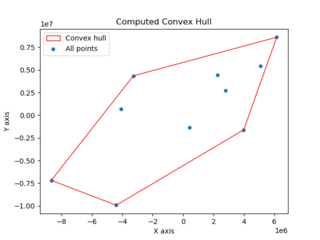
\includegraphics[width=8cm,height=8cm]{img/CH10.png}\\

\hypertarget{documentation-and-report}{%
\subsection{Documentation and Report}\label{documentation-and-report}}

Documentation of this algorithm, functions and classes can be found in
the \texttt{docs} folder in the current directory. Open the
\href{../ConvexHull/docs/html/index.html}{index.html} file from the docs
directory with your preferred browser to go through the documentation

\hypertarget{performance-analysis}{%
\subsection{Performance Analysis}\label{performance-analysis}}

Analysis is performed with a system running:

\begin{itemize}
\tightlist
\item
  OS: Arch Linux (64Bit) running Linux Kernel version 5.7.2
\item
  Processor: Intel Core i7 7700HQ
\item
  RAM: 8GB
\item
  Compiler: GNU G++ (GCC) 10.1.0
\end{itemize}

\textbf{The following observations are recorded:}

\begin{longtable}[]{@{}lcccc@{}}
\toprule
Filename & Input Dimentions & Output Diemntions & File read time &
Algorithm runtime\tabularnewline
\midrule
\endhead
edge.txt & 5 & 4 & 451 microsec & 8 microsec\tabularnewline
small.txt & 7 & 7 & 495 microsec & 16 microsec\tabularnewline
test.txt & 34 & 7 & 328 microsec & 56 microsec\tabularnewline
radial.txt & 3100 & 9 & 1348 microsec & 6.15 millisec\tabularnewline
\bottomrule
\end{longtable}

Randomly generated points (using python):

\begin{longtable}[]{@{}lcccc@{}}
\toprule
Filename & Input Dimentions & Output Diemntions & File read time &
Algorithm runtime\tabularnewline
\midrule
\endhead
10.txt & 10 & 5 & 314 microsec & 16 microsec\tabularnewline
20.txt & 20 & 7 & 495 microsec & 31 microsec\tabularnewline
50.txt & 50 & 9 & 427 microsec & 108 microsec\tabularnewline
100.txt & 100 & 13 & 348 microsec & 165 microsec\tabularnewline
500.txt & 500 & 13 & 572 microsec & 935 microsec\tabularnewline
1000.txt & 1000 (1K) & 18 & 510 microsec & 2.1 millisec\tabularnewline
3000.txt & 3000 (3K) & 24 & 2.49 millisec & 5.5 millisec\tabularnewline
5000.txt & 5000 (5K) & 22 & 2.12 millisec & 8.0 millisec\tabularnewline
10000.txt & 10000 (10K) & 23 & 3.26 millisec & 17.6
millisec\tabularnewline
50000.txt & 50000 (50K) & 28 & 17.4 millisec & 80.5
millisec\tabularnewline
100000.txt & 100000 (1L) & 31 & 39.3 millisec & 164.1
millisec\tabularnewline
250000.txt & 250000 (2.5L) & 31 & 78.1 millisec & 448.3
millisec\tabularnewline
\bottomrule
\end{longtable}

Using real world datasets:

\begin{longtable}[]{@{}lcccc@{}}
\toprule
Filename & Input Points & Output Diemntions & File read time & Algorithm
runtime\tabularnewline
\midrule
\endhead
subway-entrance-ny.txt & 1929 & 16 & 2.85 millisec & 3.81
millisec\tabularnewline
parking\_meter.txt & 15191 & 16 & 14.15 millisec & 27.04
millisec\tabularnewline
\bottomrule
\end{longtable}

Sources of datasets:

\begin{itemize}
\tightlist
\item
  \href{https://data.world/city-of-ny/5jsj-cq4s}{Parking meter dataset}
\item
  \href{https://data.world/new-york-city/subway-entrances}{New York
  Subway Entrance dataset}
\end{itemize}

It is highly difficult to calculate the time taken exactly up to the
microsecond, hence the value might vary on different executions. Also,
please note that the time calculated here may vary based on the system
load and other background applications.

\hypertarget{algorithm-approach}{%
\subsection{Algorithm Approach}\label{algorithm-approach}}

For more detailed information regarding the algorithm, refer to David
Mount Lecture notes from the course
\href{https://www.cs.umd.edu/class/spring2020/cmsc754/lectures.html}{CMSC
754 - Computational Geometry}

Given set of points P, we would like to first order them according to
the increasing x coordinate. For the sake of simplicity, let us assume
that no two points will have same x or y coordinate and no 3 points are
co-linear.

First, we will recursively compute the upper hull and then similarly
compute the lower hull of the given set of points. Finally, we will join
the upper hull with the lower hull to complete the convex hull and
return/print the clockwise ordering of the points present on the convex
hull

\textbf{Upper Hull Computation}

We divide the input set of points into 2 equal halves and recursively
compute the upper hull for both the half. Then, we compute the upper
tangent to both the hulls by traversing from the right on left hull and
traversing from left on the right hull. We perform orientation tests to
determine when the orientation changes on each hull respectively and
move upwards a point. We perform this operations until we reach the
upper part of both hulls.

All the traversed points on both hulls except the one which lead to
tangent are deleted (because all of them lie under tangent, hence lie
inside the polygon) and the resulting points of both hulls are catenated
to get the upper hull.

\hypertarget{results}{%
\subsection{Results}\label{results}}

The following is the computed convex hull of the
\href{./datasets/parking_meter.txt}{parking\_meter.txt} dataset:

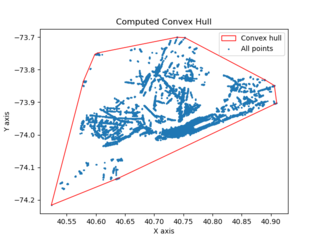
\includegraphics[width=8cm,height=8cm]{img/CHparkingmeter.png}\\

The red boundary in the above image represents the convex hull given as
the output by the program. The blue points are the inputs given to the
program.

By analysis of the above divide and conquer algorithm, It can be
concluded that the algorithm runs in O(n log n) time complexity. From
the above results of testing of various datasets, we can see that the
time increase is proportional to the no of points.

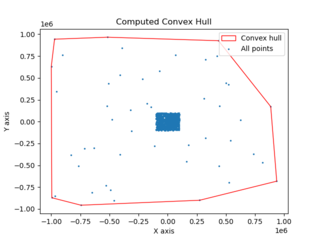
\includegraphics[width=8cm,height=8cm]{img/CHradial.png}\\

The dataset \href{./datasets/radial.txt}{radial.txt} is a hand-crafted
dataset (3K points) which has high concentration of points
(\textasciitilde2.1K) in the center, whereas other randomly generated
datasets (for example: \href{./datasets/3000.txt}{3000.txt})have a
uniform distribution of points (the python random number generator uses
an underlying uniform distribution). From this we can assume that
independant of positioning of points, our algorithm takes approximately
the same time to compute the convex hull.

\hypertarget{conclusion}{%
\subsection{Conclusion}\label{conclusion}}

For the last dataset which contains 2.5L points, its worth noting that
the algorithm runs in just under 500ms which might appear to be fast.
But for applications like graphics, rendering and animations, this poses
a huge overhead in terms of repeated computation of convex hull for
various objects.

One observation we can make here is that the number of points which are
present on the convex hull is usually relatively lower most of the
times. So, using an output sensitive algorithms (Ex: Jarvis's march)
might help us if our application has fewer vertices on the convex hull.

It's worth noting that convex hull computation cannot be done under O(n
log n) which has been proved. Therefore, we can only hope to reduce the
constants of complexity. In our algorithm, we repeatedly recurse, hence
make many function calls which is computationally expensive. Hence by
using algorithms like Chan's or Grahm's, we can do better

\hypertarget{dcel---doubly-connected-edge-list}{%
\section{DCEL - Doubly Connected Edge
List}\label{dcel---doubly-connected-edge-list}}

\hypertarget{introduction}{%
\subsection{Introduction}\label{introduction}}

Doubly connected edge list (DCEL), which is also known as halfedge data
structure, is used to efficiently represent planar graphs. Using a DCEL
structure, we can easily manipulate the topological information of the
planar graph such as vertices, faces and edges.

In general, a DCEL conatins a book-keeping record of all edges, vertices
and faces of the graph. Each record individually can contain information
of all it's incident geometric objects. We will look at how a DCEL
stores this information in
\protect\hyperlink{data-structure-approach}{Data Structure Approach}
section.

\hypertarget{how-to-run}{%
\subsection{How to Run}\label{how-to-run}}

The src folder contains the source code for the DCEL data structure.
\texttt{g++} from the GNU compiler suite is required to compile the
program to a executable.

Steps to Compile:

\begin{enumerate}
\def\labelenumi{\arabic{enumi})}
\tightlist
\item
  \texttt{cd} into the src directory
\item
  Run \texttt{g++\ main.cpp} which generates an executable called
  \texttt{a.out} in the same directory
\item
  Run the executable using \texttt{./a.out} (on linux)

  \begin{enumerate}
  \def\labelenumii{\arabic{enumii})}
  \tightlist
  \item
    The executable takes a dataset from command line argument. For
    example, to use an existing dataset, run
    \texttt{./a.out\ ../datasets/1sq.txt}
  \item
    If no command-line argument is given, it takes input from the shell
    directly (stdin)
  \end{enumerate}
\end{enumerate}

\hypertarget{input}{%
\subsection{Input}\label{input}}

The required input format for the algorithm to work correctly is:

\begin{itemize}
\tightlist
\item
  Input can be given both from file (via command-line args) or stdin
\item
  First line must contain the no of Edges to be taken as input by the
  program.
\item
  Each of next line must contain 4 integers, space seperated denoting
  the (x1, y1), (x2, y2) coordinates of endpoints of each edge.
\item
  Each coordinate must be of integer type in the range -10\^{}8 to
  10\^{}8.
\item
  Number of coordinates must be less than 1 Billion.
\end{itemize}

\hypertarget{output}{%
\subsection{Output}\label{output}}

Output of the algorithm prints all the HalfEdges incident to each face
by traversing its representative half edges. All the faces outputed by
the program can also be verified by running it through the plotting
diagram.\\
The last two lines of output show the time taken to take input in
microseconds and the time taken by the algorithm to compute DCEL (also
in microseconds).

An example of output of dataset
\href{./datasets/random4.txt}{random4.txt}:

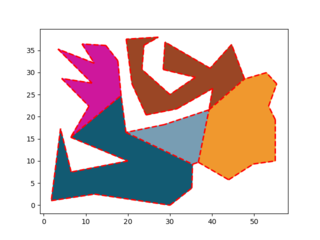
\includegraphics[width=8cm,height=8cm]{img/DCELrandom.png}\\

\hypertarget{documentation-and-report}{%
\subsection{Documentation and Report}\label{documentation-and-report}}

Documentation of this algorithm, functions and classes can be found in
the \texttt{docs} folder in the current directory. Open the
\href{../DCEL/docs/html/index.html}{index.html} file from the docs
directory with your preferred browser to go through the documentation

\hypertarget{performance-analysis}{%
\subsection{Performance Analysis}\label{performance-analysis}}

This analysis does not include the time taken to show output on
terminal. Analysis is performed with a system running:

\begin{itemize}
\tightlist
\item
  OS: Arch Linux (64Bit) running Linux Kernel version 5.7.2
\item
  Processor: Intel Core i7 7700HQ
\item
  RAM: 8GB
\item
  Compiler: GNU G++ (GCC) 10.1.0
\end{itemize}

\textbf{The following observations are recorded:}

Manual generated test files:

\begin{longtable}[]{@{}lccccc@{}}
\toprule
\begin{minipage}[b]{0.12\columnwidth}\raggedright
Filename\strut
\end{minipage} & \begin{minipage}[b]{0.15\columnwidth}\centering
Input Vertices\strut
\end{minipage} & \begin{minipage}[b]{0.12\columnwidth}\centering
Input Edges\strut
\end{minipage} & \begin{minipage}[b]{0.12\columnwidth}\centering
Input Faces\strut
\end{minipage} & \begin{minipage}[b]{0.15\columnwidth}\centering
File read time\strut
\end{minipage} & \begin{minipage}[b]{0.17\columnwidth}\centering
DCEL Creation Time\strut
\end{minipage}\tabularnewline
\midrule
\endhead
\begin{minipage}[t]{0.12\columnwidth}\raggedright
1sq.txt\strut
\end{minipage} & \begin{minipage}[t]{0.15\columnwidth}\centering
4\strut
\end{minipage} & \begin{minipage}[t]{0.12\columnwidth}\centering
4\strut
\end{minipage} & \begin{minipage}[t]{0.12\columnwidth}\centering
2\strut
\end{minipage} & \begin{minipage}[t]{0.15\columnwidth}\centering
505 microsec\strut
\end{minipage} & \begin{minipage}[t]{0.17\columnwidth}\centering
27 microsec\strut
\end{minipage}\tabularnewline
\begin{minipage}[t]{0.12\columnwidth}\raggedright
4sq.txt\strut
\end{minipage} & \begin{minipage}[t]{0.15\columnwidth}\centering
9\strut
\end{minipage} & \begin{minipage}[t]{0.12\columnwidth}\centering
12\strut
\end{minipage} & \begin{minipage}[t]{0.12\columnwidth}\centering
5\strut
\end{minipage} & \begin{minipage}[t]{0.15\columnwidth}\centering
396 microsec\strut
\end{minipage} & \begin{minipage}[t]{0.17\columnwidth}\centering
46 microsec\strut
\end{minipage}\tabularnewline
\begin{minipage}[t]{0.12\columnwidth}\raggedright
random1.txt\strut
\end{minipage} & \begin{minipage}[t]{0.15\columnwidth}\centering
10\strut
\end{minipage} & \begin{minipage}[t]{0.12\columnwidth}\centering
12\strut
\end{minipage} & \begin{minipage}[t]{0.12\columnwidth}\centering
4\strut
\end{minipage} & \begin{minipage}[t]{0.15\columnwidth}\centering
257 microsec\strut
\end{minipage} & \begin{minipage}[t]{0.17\columnwidth}\centering
52 microsec\strut
\end{minipage}\tabularnewline
\begin{minipage}[t]{0.12\columnwidth}\raggedright
random3.txt\strut
\end{minipage} & \begin{minipage}[t]{0.15\columnwidth}\centering
23\strut
\end{minipage} & \begin{minipage}[t]{0.12\columnwidth}\centering
26\strut
\end{minipage} & \begin{minipage}[t]{0.12\columnwidth}\centering
5\strut
\end{minipage} & \begin{minipage}[t]{0.15\columnwidth}\centering
175 microsec\strut
\end{minipage} & \begin{minipage}[t]{0.17\columnwidth}\centering
84 microsec\strut
\end{minipage}\tabularnewline
\begin{minipage}[t]{0.12\columnwidth}\raggedright
random2.txt\strut
\end{minipage} & \begin{minipage}[t]{0.15\columnwidth}\centering
23\strut
\end{minipage} & \begin{minipage}[t]{0.12\columnwidth}\centering
37\strut
\end{minipage} & \begin{minipage}[t]{0.12\columnwidth}\centering
16\strut
\end{minipage} & \begin{minipage}[t]{0.15\columnwidth}\centering
192 microsec\strut
\end{minipage} & \begin{minipage}[t]{0.17\columnwidth}\centering
102 microsec\strut
\end{minipage}\tabularnewline
\begin{minipage}[t]{0.12\columnwidth}\raggedright
a.txt\strut
\end{minipage} & \begin{minipage}[t]{0.15\columnwidth}\centering
31\strut
\end{minipage} & \begin{minipage}[t]{0.12\columnwidth}\centering
33\strut
\end{minipage} & \begin{minipage}[t]{0.12\columnwidth}\centering
4\strut
\end{minipage} & \begin{minipage}[t]{0.15\columnwidth}\centering
150 microsec\strut
\end{minipage} & \begin{minipage}[t]{0.17\columnwidth}\centering
109 microsec\strut
\end{minipage}\tabularnewline
\begin{minipage}[t]{0.12\columnwidth}\raggedright
random4.txt\strut
\end{minipage} & \begin{minipage}[t]{0.15\columnwidth}\centering
44\strut
\end{minipage} & \begin{minipage}[t]{0.12\columnwidth}\centering
48\strut
\end{minipage} & \begin{minipage}[t]{0.12\columnwidth}\centering
6\strut
\end{minipage} & \begin{minipage}[t]{0.15\columnwidth}\centering
364 microsec\strut
\end{minipage} & \begin{minipage}[t]{0.17\columnwidth}\centering
165 microsec\strut
\end{minipage}\tabularnewline
\begin{minipage}[t]{0.12\columnwidth}\raggedright
house.txt\strut
\end{minipage} & \begin{minipage}[t]{0.15\columnwidth}\centering
71\strut
\end{minipage} & \begin{minipage}[t]{0.12\columnwidth}\centering
81\strut
\end{minipage} & \begin{minipage}[t]{0.12\columnwidth}\centering
12\strut
\end{minipage} & \begin{minipage}[t]{0.15\columnwidth}\centering
250 microsec\strut
\end{minipage} & \begin{minipage}[t]{0.17\columnwidth}\centering
300 microsec\strut
\end{minipage}\tabularnewline
\bottomrule
\end{longtable}

Using real world datasets:

\begin{itemize}
\tightlist
\item
  Road network of hyderabad, source: GPS coordinates filtered from
  osm(openstreetmap) data on hyderabad

  \begin{itemize}
  \tightlist
  \item
    hyd\_1.txt: contains road network having tag of \emph{highway} set
    as `trunk'
  \item
    hyd\_2.txt: contains road network having tag of \emph{highway} set
    as `trunk' and `primary'
  \item
    hyd\_2.txt: contains road network having tag of \emph{highway} set
    as `trunk', `primary' and `secondary'
  \item
    hyd\_2.txt: contains road network having tag of \emph{highway} set
    as `trunk', `primary', `secondary', and `motorway'
  \end{itemize}
\end{itemize}

\begin{longtable}[]{@{}lccccc@{}}
\toprule
\begin{minipage}[b]{0.12\columnwidth}\raggedright
Filename\strut
\end{minipage} & \begin{minipage}[b]{0.15\columnwidth}\centering
Input Vertices\strut
\end{minipage} & \begin{minipage}[b]{0.12\columnwidth}\centering
Input Edges\strut
\end{minipage} & \begin{minipage}[b]{0.12\columnwidth}\centering
Input Faces\strut
\end{minipage} & \begin{minipage}[b]{0.15\columnwidth}\centering
File read time\strut
\end{minipage} & \begin{minipage}[b]{0.17\columnwidth}\centering
Algorithm runtime\strut
\end{minipage}\tabularnewline
\midrule
\endhead
\begin{minipage}[t]{0.12\columnwidth}\raggedright
hyd\_1.txt\strut
\end{minipage} & \begin{minipage}[t]{0.15\columnwidth}\centering
685\strut
\end{minipage} & \begin{minipage}[t]{0.12\columnwidth}\centering
733\strut
\end{minipage} & \begin{minipage}[t]{0.12\columnwidth}\centering
58\strut
\end{minipage} & \begin{minipage}[t]{0.15\columnwidth}\centering
2.4 millisec\strut
\end{minipage} & \begin{minipage}[t]{0.17\columnwidth}\centering
1.68 millisec\strut
\end{minipage}\tabularnewline
\begin{minipage}[t]{0.12\columnwidth}\raggedright
hyd\_2.txt\strut
\end{minipage} & \begin{minipage}[t]{0.15\columnwidth}\centering
1787\strut
\end{minipage} & \begin{minipage}[t]{0.12\columnwidth}\centering
1912\strut
\end{minipage} & \begin{minipage}[t]{0.12\columnwidth}\centering
229\strut
\end{minipage} & \begin{minipage}[t]{0.15\columnwidth}\centering
3.5 millisec\strut
\end{minipage} & \begin{minipage}[t]{0.17\columnwidth}\centering
107.5 millisec\strut
\end{minipage}\tabularnewline
\begin{minipage}[t]{0.12\columnwidth}\raggedright
hyd\_3.txt\strut
\end{minipage} & \begin{minipage}[t]{0.15\columnwidth}\centering
2959\strut
\end{minipage} & \begin{minipage}[t]{0.12\columnwidth}\centering
3198\strut
\end{minipage} & \begin{minipage}[t]{0.12\columnwidth}\centering
519\strut
\end{minipage} & \begin{minipage}[t]{0.15\columnwidth}\centering
5.4 millisec\strut
\end{minipage} & \begin{minipage}[t]{0.17\columnwidth}\centering
276.9 millisec\strut
\end{minipage}\tabularnewline
\begin{minipage}[t]{0.12\columnwidth}\raggedright
hyd\_4.txt\strut
\end{minipage} & \begin{minipage}[t]{0.15\columnwidth}\centering
3612\strut
\end{minipage} & \begin{minipage}[t]{0.12\columnwidth}\centering
3850\strut
\end{minipage} & \begin{minipage}[t]{0.12\columnwidth}\centering
532\strut
\end{minipage} & \begin{minipage}[t]{0.15\columnwidth}\centering
24.3 millisec\strut
\end{minipage} & \begin{minipage}[t]{0.17\columnwidth}\centering
337.8 millisec\strut
\end{minipage}\tabularnewline
\bottomrule
\end{longtable}

\hypertarget{data-structure-approach}{%
\subsection{Data Structure Approach}\label{data-structure-approach}}

The following geometric objects are used in DCEL:

\begin{itemize}
\tightlist
\item
  \textbf{Vertex}: Object to store vertex coordinates and any one of its
  incident halfedges as its representative.
\item
  \textbf{Edge}: Object to store its vertex endpoints.
\item
  \textbf{Face}: Object to store a unique face-id and one of its
  incident halfedges as its representative
\item
  \textbf{HalfEdge}: Object to store a directed halfedge which has
  pointers to all its incident geometric objects (Vertex, Face, next and
  previous halfedges and its twin halfedge)
\end{itemize}

This implementation uses a Hash Map to store list of all incident
halfedges for each vertex. This Hash Map uses vertex pointer as key and
stores a list of halfedges as value. Our DCEL also has a list of
Vertices and Faces which can be used to iterate through all Vertices and
Faces quickly.

A half-edge has a pointer to the next half-edge and previous half-edge
of the same face. Each half-edge has a single face as its representative
Face (which is present towards left side of it). All half-edges
associated with a face are counter-clockwise which can be obtained by
traversing its representative Halfedge. To reach the other face, we can
go to the twin of the half-edge and then traverse the other face. Each
half-edge also has a pointer to its origin vertex which can be used to
get all the Vertex points of the corresponding face.

\hypertarget{results}{%
\subsection{Results}\label{results}}

This algorithm to construct a DCEL takes time complexity of O(V+E). From
the analysis of example dataset runtimes, we can easily see that
increase in number of vertices and edges directly leads to increase in
DCEL construction time.

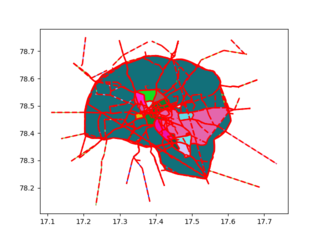
\includegraphics[width=8cm,height=8cm]{img/DCELhyd4.png}\\

The output of the algorithm is direct traversal of representative edges
of all faces present in the input. In the above example of Hyderabad
road network dataset, it shows all the faces bounded by the roads. All
faces might not be visible directly as the road system branches without
forming many faces. But as we zoom, the faces can be spotted between
roads.

\hypertarget{conclusion}{%
\subsection{Conclusion}\label{conclusion}}

The time complexity O(V+E) cannot be reduced further because to store
the graph, it is required to traverse through all Vertices and Edges
present in the graph. Although the current implementation only supports
connected graphs, it can also be extended to store disconnected
components using techniques like hidden vertices.

From the above results, we can be sure that DCEL can be a good candidate
data structure for easy representation of planar graphs. But as every
other data structure, even DCEL has it downfalls. The main one being the
amount of Storage required to store. The storage requirement can be
further reduced if we only need to store Vertices or Edges, but this
does not give huge improvements. Also, as the size of DCEL increases,
the time to add an extra edge increases in a linear fashion which might
be bad based on the application.DCEL is a simple data structure which
helps to easily manupulate the graph structre, but it might not be an
appropriate choice for low memory applications such as in embedded
systems.

\hypertarget{polygon-triangulation}{%
\section{Polygon Triangulation}\label{polygon-triangulation}}

\hypertarget{introduction}{%
\subsection{Introduction}\label{introduction}}

The decomposition of a polygon into triangles whose union again results
in the original polygon is called polygon triangulation. In the method,
no new Vertices are added. Only the diagonals of the polygon results in
the triangulation. There need not be a unique triangulation for a given
polygon.

There are various methods which can be used to perform polygon
triangulation. In our implementation, we
\protect\hyperlink{algorithm-approach}{discuss} two types of
triangulation which are: 1) Ear Clipping Triangulation. 2) Plane sweep
monotone division combined with Monotone triangulation.

\hypertarget{how-to-run}{%
\subsection{How to Run}\label{how-to-run}}

The src folder contains the source code for the convex hull program.
\texttt{g++} from the GNU compiler suite is required to compile the
program to a executable.

Steps to Compile:

\begin{enumerate}
\def\labelenumi{\arabic{enumi})}
\tightlist
\item
  \texttt{cd} into the src directory
\item
  Run \texttt{g++\ main.cpp} which generates an executable called
  \texttt{a.out} in the same directory
\item
  Run the executable using \texttt{./a.out} (on linux)

  \begin{enumerate}
  \def\labelenumii{\arabic{enumii})}
  \tightlist
  \item
    The executable takes a dataset from command line argument. For
    example, to use an existing dataset, run
    \texttt{./a.out\ ../datasets/complex.txt}
  \item
    If no command-line argument is given, it takes input from the shell
    directly (stdin)
  \end{enumerate}
\end{enumerate}

\hypertarget{input}{%
\subsection{Input}\label{input}}

The required file format for the algorithm to work correctly is:

\begin{itemize}
\tightlist
\item
  The input \textbf{must} be a clockwise ordering of Poins present on
  the polygon.
\item
  First line must contain the no of Points to be taken as input by the
  program.
\item
  Each of next line must contain 2 integers, space seperated denoting
  the (x, y) coordinates of each point.
\item
  Each coordinate must be of integer type in the range -10\^{}8 to
  10\^{}8.
\item
  No of coordinates must be less than 1 Billion.
\end{itemize}

\hypertarget{output}{%
\subsection{Output}\label{output}}

Each line of output contains three coordinates of points present on each
triangulation.\\
The last two lines of output show the time taken to take input in
microseconds and the time taken by the algorithm to compute
Triangulation (also in microseconds).

This is the output of one of the datasets
\href{./datasets/long.txt}{long.txt}

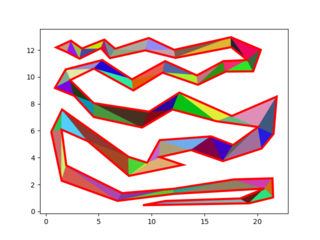
\includegraphics[width=8cm,height=8cm]{img/TRIsnake.png}\\

\hypertarget{documentation-and-report}{%
\subsection{Documentation and Report}\label{documentation-and-report}}

Documentation of this algorithm, functions and classes can be found in
the \texttt{docs} folder in the current directory. Open the
\href{../Triangulation/docs/html/index.html}{index.html} file from the
docs directory with your preferred browser to go through the
documentation

\hypertarget{performance-analysis}{%
\subsection{Performance Analysis}\label{performance-analysis}}

Analysis is performed with a system running (does not include printing
time):

\begin{itemize}
\tightlist
\item
  OS: Arch Linux (64Bit) running Linux Kernel version 5.7.2
\item
  Processor: Intel Core i7 7700HQ
\item
  RAM: 8GB
\item
  Compiler: GNU G++ (GCC) 10.1.0
\end{itemize}

\textbf{The following observations are recorded:}

Time taken to triangulate basic shapes:

\begin{longtable}[]{@{}lcccc@{}}
\toprule
\begin{minipage}[b]{0.07\columnwidth}\raggedright
Filename\strut
\end{minipage} & \begin{minipage}[b]{0.12\columnwidth}\centering
Input Vertices\strut
\end{minipage} & \begin{minipage}[b]{0.15\columnwidth}\centering
Computed Triangles\strut
\end{minipage} & \begin{minipage}[b]{0.25\columnwidth}\centering
Line Sweep Triangulation Runtime\strut
\end{minipage} & \begin{minipage}[b]{0.27\columnwidth}\centering
Ear Clipping Triangulation Runtime\strut
\end{minipage}\tabularnewline
\midrule
\endhead
\begin{minipage}[t]{0.07\columnwidth}\raggedright
triangle.txt\strut
\end{minipage} & \begin{minipage}[t]{0.12\columnwidth}\centering
3\strut
\end{minipage} & \begin{minipage}[t]{0.15\columnwidth}\centering
1\strut
\end{minipage} & \begin{minipage}[t]{0.25\columnwidth}\centering
30 microsec\strut
\end{minipage} & \begin{minipage}[t]{0.27\columnwidth}\centering
16 microsec\strut
\end{minipage}\tabularnewline
\begin{minipage}[t]{0.07\columnwidth}\raggedright
downConvex.txt\strut
\end{minipage} & \begin{minipage}[t]{0.12\columnwidth}\centering
6\strut
\end{minipage} & \begin{minipage}[t]{0.15\columnwidth}\centering
4\strut
\end{minipage} & \begin{minipage}[t]{0.25\columnwidth}\centering
43 microsec\strut
\end{minipage} & \begin{minipage}[t]{0.27\columnwidth}\centering
23 microsec\strut
\end{minipage}\tabularnewline
\begin{minipage}[t]{0.07\columnwidth}\raggedright
test.txt\strut
\end{minipage} & \begin{minipage}[t]{0.12\columnwidth}\centering
6\strut
\end{minipage} & \begin{minipage}[t]{0.15\columnwidth}\centering
4\strut
\end{minipage} & \begin{minipage}[t]{0.25\columnwidth}\centering
35 microsec\strut
\end{minipage} & \begin{minipage}[t]{0.27\columnwidth}\centering
24 microsec\strut
\end{minipage}\tabularnewline
\begin{minipage}[t]{0.07\columnwidth}\raggedright
square.txt\strut
\end{minipage} & \begin{minipage}[t]{0.12\columnwidth}\centering
4\strut
\end{minipage} & \begin{minipage}[t]{0.15\columnwidth}\centering
2\strut
\end{minipage} & \begin{minipage}[t]{0.25\columnwidth}\centering
36 microsec\strut
\end{minipage} & \begin{minipage}[t]{0.27\columnwidth}\centering
18 microsec\strut
\end{minipage}\tabularnewline
\begin{minipage}[t]{0.07\columnwidth}\raggedright
hexagon.txt\strut
\end{minipage} & \begin{minipage}[t]{0.12\columnwidth}\centering
6\strut
\end{minipage} & \begin{minipage}[t]{0.15\columnwidth}\centering
4\strut
\end{minipage} & \begin{minipage}[t]{0.25\columnwidth}\centering
38 microsec\strut
\end{minipage} & \begin{minipage}[t]{0.27\columnwidth}\centering
16 microsec\strut
\end{minipage}\tabularnewline
\begin{minipage}[t]{0.07\columnwidth}\raggedright
monotone.txt\strut
\end{minipage} & \begin{minipage}[t]{0.12\columnwidth}\centering
15\strut
\end{minipage} & \begin{minipage}[t]{0.15\columnwidth}\centering
13\strut
\end{minipage} & \begin{minipage}[t]{0.25\columnwidth}\centering
109 microsec\strut
\end{minipage} & \begin{minipage}[t]{0.27\columnwidth}\centering
75 microsec\strut
\end{minipage}\tabularnewline
\begin{minipage}[t]{0.07\columnwidth}\raggedright
uniMonotone.txt\strut
\end{minipage} & \begin{minipage}[t]{0.12\columnwidth}\centering
8\strut
\end{minipage} & \begin{minipage}[t]{0.15\columnwidth}\centering
6\strut
\end{minipage} & \begin{minipage}[t]{0.25\columnwidth}\centering
115 microsec\strut
\end{minipage} & \begin{minipage}[t]{0.27\columnwidth}\centering
42 microsec\strut
\end{minipage}\tabularnewline
\begin{minipage}[t]{0.07\columnwidth}\raggedright
complex.txt\strut
\end{minipage} & \begin{minipage}[t]{0.12\columnwidth}\centering
17\strut
\end{minipage} & \begin{minipage}[t]{0.15\columnwidth}\centering
15\strut
\end{minipage} & \begin{minipage}[t]{0.25\columnwidth}\centering
188 microsec\strut
\end{minipage} & \begin{minipage}[t]{0.27\columnwidth}\centering
17 microsec\strut
\end{minipage}\tabularnewline
\begin{minipage}[t]{0.07\columnwidth}\raggedright
strange.txt\strut
\end{minipage} & \begin{minipage}[t]{0.12\columnwidth}\centering
16\strut
\end{minipage} & \begin{minipage}[t]{0.15\columnwidth}\centering
14\strut
\end{minipage} & \begin{minipage}[t]{0.25\columnwidth}\centering
148 microsec\strut
\end{minipage} & \begin{minipage}[t]{0.27\columnwidth}\centering
122 microsec\strut
\end{minipage}\tabularnewline
\begin{minipage}[t]{0.07\columnwidth}\raggedright
star.txt\strut
\end{minipage} & \begin{minipage}[t]{0.12\columnwidth}\centering
10\strut
\end{minipage} & \begin{minipage}[t]{0.15\columnwidth}\centering
8\strut
\end{minipage} & \begin{minipage}[t]{0.25\columnwidth}\centering
159 microsec\strut
\end{minipage} & \begin{minipage}[t]{0.27\columnwidth}\centering
101 microsec\strut
\end{minipage}\tabularnewline
\begin{minipage}[t]{0.07\columnwidth}\raggedright
spiral.txt\strut
\end{minipage} & \begin{minipage}[t]{0.12\columnwidth}\centering
32\strut
\end{minipage} & \begin{minipage}[t]{0.15\columnwidth}\centering
30\strut
\end{minipage} & \begin{minipage}[t]{0.25\columnwidth}\centering
278 microsec\strut
\end{minipage} & \begin{minipage}[t]{0.27\columnwidth}\centering
214 microsec\strut
\end{minipage}\tabularnewline
\begin{minipage}[t]{0.07\columnwidth}\raggedright
tank.txt\strut
\end{minipage} & \begin{minipage}[t]{0.12\columnwidth}\centering
55\strut
\end{minipage} & \begin{minipage}[t]{0.15\columnwidth}\centering
53\strut
\end{minipage} & \begin{minipage}[t]{0.25\columnwidth}\centering
429 microsec\strut
\end{minipage} & \begin{minipage}[t]{0.27\columnwidth}\centering
452 microsec\strut
\end{minipage}\tabularnewline
\begin{minipage}[t]{0.07\columnwidth}\raggedright
long.txt\strut
\end{minipage} & \begin{minipage}[t]{0.12\columnwidth}\centering
72\strut
\end{minipage} & \begin{minipage}[t]{0.15\columnwidth}\centering
70\strut
\end{minipage} & \begin{minipage}[t]{0.25\columnwidth}\centering
593 microsec\strut
\end{minipage} & \begin{minipage}[t]{0.27\columnwidth}\centering
1668 microsec\strut
\end{minipage}\tabularnewline
\bottomrule
\end{longtable}

\hypertarget{algorithm-approach}{%
\subsection{Algorithm Approach}\label{algorithm-approach}}

\hypertarget{ear-clipping}{%
\subsubsection{Ear Clipping}\label{ear-clipping}}

According to the two ears theorem, any simple polygon with minimum of 4
vertices without holes has atleast two ``ears''. An Ear is defined at
the vertex where internal angle is less than PI and the line joining the
adjacent vertices is a diagonal of the polygon.

The algorithm works by removing away these ``ears'' (which are
triangles) until the complete polygon is triangulated. This algorithm is
easy to implement, but slower than some other algorithms, and it only
works on polygons without holes. The runtime complexity of this
algorithm is O(n\textsuperscript{2})

\hypertarget{plane-sweep-monotone-triangulation}{%
\subsubsection{Plane Sweep Monotone
Triangulation}\label{plane-sweep-monotone-triangulation}}

A monotone polygon can be easily triangulated in O(n) complexity. A
simple polygon is said to be monotone w.r.t a line L only if any line
perpendicular to L passes through the polygon at most twice. Any
monotone polygon can be divided into two monotone chains. A polygon that
is monotone w.r.t the x-axis is called x-monotone. Given x-monotone
polygon, the greedy algorithm begins by walking on one chain of the
polygon from top to bottom while adding diagonals (forming triangles)
whenever it is possible.

If a polygon is not monotone, it can be partitioned into monotone sub
polygons in O(n log n) time using line/plane sweep method. Generally,
this algorithm can triangulate a planar subdivision with in O(n log n)
time using O(n) space.

\hypertarget{results}{%
\subsection{Results}\label{results}}

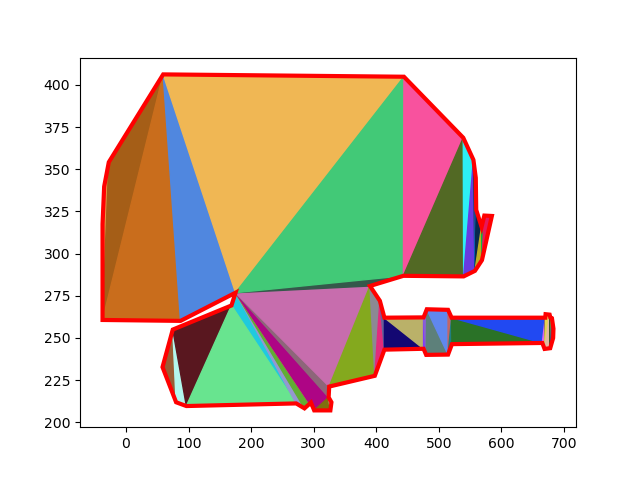
\includegraphics[width=8cm,height=8cm]{img/TRItank.png}\\

In the above image, the red boundary represents the input given to the
algorithm and the random colored triangle represent the output given by
the program.

It can be observed from the examples that increase in number of vertices
affects the runtime of ear clipping triangulation more than the plane
sweep monotone triangulation. From the results of the above datasets, we
can see that for just an increase of vertices from 50 to 70 causes the
ear clipping algorithm to triple its triangulation time.

\hypertarget{conclusion}{%
\subsection{Conclusion}\label{conclusion}}

From the above comparisions, we can see that ear clipping algorithm,
even after being a simple algorithm, due it is asymptotic complexity
being O(n\textsuperscript{2}), it surely is not recomended for
applications where number of vertices go beyond 70 (which almost always
happens).

If we know that the input only has a monotone polygon, it is even more
easier and faster to triangulate it in just O(n). The main plane sweep
algorithm tries to use this to its advantage by dividing the polygon
first into monotones.


\end{document}
